%\documentclass[a4paper]{article}
\usepackage[utf8]{inputenc}
\usepackage[spanish, es-tabla, es-noshorthands]{babel}
\usepackage[table,xcdraw]{xcolor}
\usepackage[a4paper, footnotesep=1.25cm, headheight=1.25cm, top=2.54cm, left=2.54cm, bottom=2.54cm, right=2.54cm]{geometry}
%\geometry{showframe}

%\usepackage{wrapfig}			%Wrap figure in text
\usepackage[export]{adjustbox}	%Move images
\usepackage{changepage}			%Move tables

\usepackage{tikz}
\usepackage{amsmath}
\usepackage{amsfonts}
\usepackage{amssymb}
\usepackage{float}
\usepackage{graphicx}
\usepackage{caption}
\usepackage{subcaption}
\usepackage{multicol}
\usepackage{multirow}
\usepackage{wrapfig}
\setlength{\doublerulesep}{\arrayrulewidth}
\usepackage{booktabs}
\usepackage[numbib, nottoc, notlot, notlof]{tocbibind}

\usepackage{hyperref}
\hypersetup{
    colorlinks=true,
    linkcolor=blue,
    filecolor=magenta,      
    urlcolor=blue,
    citecolor=blue,    
}

%Change Font Size

% #1 = size, #2 = text
\newcommand{\setparagraphsize}[2]{{\fontsize{#1}{6}\selectfont#2 \par}}		%Cambia el size de todo el parrafo
\newcommand{\setlinesize}[2]{{\fontsize{#1}{6}\selectfont#2}}				%Cambia el font de una oración

\newcommand{\note}[1]{
	\begin{center}
		\huge{ \textcolor{red}{#1} }
	\end{center}
}

%FONTS (IMPORTANTE): Compilar en XeLaTex o LuaLaTeX
\usepackage{anyfontsize}	%Font size
\usepackage{fontspec}		%Font type

\usepackage{etoolbox}
\usepackage{todonotes}

\newcommand{\observacion}[2]{  \ifnumequal{1}{#1}{ { \todo[inline,backgroundcolor=red!25,bordercolor=red!100]{\textbf{Observación: #2}} } }{  }  }

\setcounter{topnumber}{2}
\setcounter{bottomnumber}{2}
\setcounter{totalnumber}{4}
\renewcommand{\topfraction}{0.85}
\renewcommand{\bottomfraction}{0.85}
\renewcommand{\textfraction}{0.15}
\renewcommand{\floatpagefraction}{0.8}
\renewcommand{\textfraction}{0.1}
\setlength{\floatsep}{5pt plus 2pt minus 2pt}
\setlength{\textfloatsep}{5pt plus 2pt minus 2pt}
\setlength{\intextsep}{5pt plus 2pt minus 2pt}

\newcommand{\quotes}[1]{``#1''}
\usepackage{array}
\newcolumntype{C}[1]{>{\centering\let\newline\\\arraybackslash\hspace{0pt}}m{#1}}
\usepackage[american]{circuitikz}
\usetikzlibrary{calc}
\usepackage{fancyhdr}
\usepackage{units} 

\graphicspath{{../Control de posición no lineal/}{../Control de fuerza no lineal/}{../Control híbrido no lineal/}{../Referencias/}{../Deducción de modelo/}{../Conclusiones/}}

\pagestyle{fancy}
\fancyhf{}
\lhead{22.99 - Automación Industrial}
\rhead{Lambertucci, Londero B., Maselli, Mechoulam}
\rfoot{Página \thepage}

%Items con bullets y no cuadrados
\renewcommand{\labelitemi}{\textbullet }


%\begin{document}

La consigna propone un manipulador RR de las siguientes cualidades.
\begin{figure}[H]
	\centering
	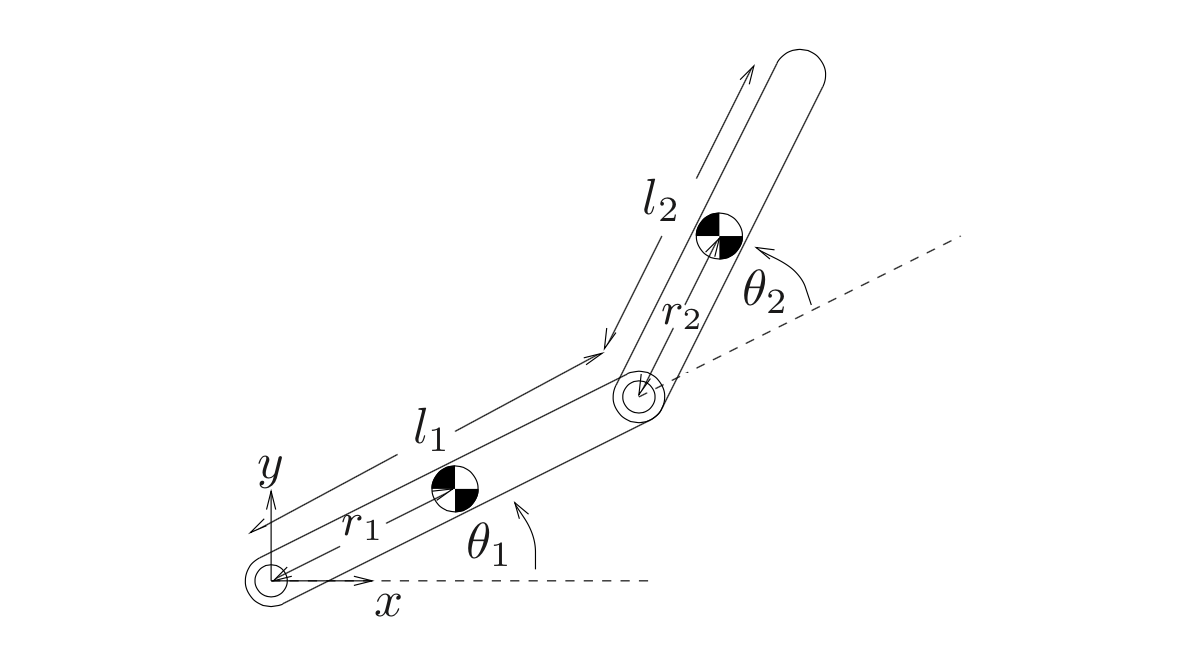
\includegraphics[width=0.8\linewidth]{ImagenesDeducción de modelo/brazo}
	\caption{Manipulador RR.}	
	\label{fig:brazo}
\end{figure}
Donde para los parametros DH se opto por la posicion $\theta_1 \ = \ 0$ y $\theta_2 \ = \ 0$.
A partir de ello se obtuvieron los siguientes par\'ametros DH (Donde todas las ternas son paralelas. Los Z paralelos, los ejes X colineales y en sentido del siguiente link).
\begin{table}[H]
\centering
\begin{tabular}{c|c|c|c|c}
\textbf{}   & \textbf{$\alpha$} & \textbf{a} & \textbf{$\theta$} & \textbf{d} \\ \hline
\textbf{1}  & 0                 & 0          & $\theta_1$        & 0          \\
\textbf{2}  & 0                 & $L_1$      & $\theta_2$        & 0          \\
\textbf{EE} & 0                 & $L_2$      & 0                 & 0          \\ \hline
\end{tabular}
\end{table}
Luego realizando la propagaci\'on de velocidades se obtiene que:
\begin{equation}
^1v_1 = 0 
\end{equation}
\begin{equation}
^1\omega_1= \dot{\theta_1} \ \cdot \ \hat{k}
\end{equation}
\begin{equation}
^2v_2 = \dot{\theta_1} \cdot \sin(\theta_2)L \  \cdot \ \hat{i} + \dot{\theta_1} \cdot \cos(\theta_2)L  \ \cdot \  \hat{j}
\end{equation}

\begin{equation}
^2\omega_2= \dot{\theta_1}+\dot{\theta_2}  \ \cdot \ \hat{k}
\end{equation}
Luego obteniendo los correspondientes a los centros de masa (Ubicados al final de cada link).
\begin{equation}
^1v_{c1}=\dot{\theta_1}L \ \cdot \  \hat{j}
\end{equation}

\begin{equation}
^2v_{c2}=\dot{\theta_1} \cdot \sin(\theta_2)L  \ \cdot \ \hat{i} + \left( \dot{\theta_1} \cdot \cos(\theta_2)L  + L( \dot{\theta_1}+\dot{\theta_2} ) \right) \ \cdot \  \hat{j}
\end{equation}
Las matrices de inercia ser\'an diagonales con valores $I_{zz}=mL^2$, $I_{yy}=mL^2$ e $I_{xx}=0$


Luego se procede a calcular el vector de torques.
\begin{equation}
\mathcal{L}(\Theta , \dot{\Theta}) = k(\Theta , \dot{\Theta}) - u(\Theta)
\end{equation}
\begin{equation}
\tau = \frac{d}{dt}\left(\frac{\partial k}{\partial \dot{\Theta}} \right) - \frac{\partial k}{\partial \Theta} + \frac{\partial u}{\partial \Theta}
\end{equation}
Debido a que todo el movimiento del brazo se encuentra al mismo potencial gravitatorio los terminos de u son nulos.


Operando se obtiene un modelo de la siguiente forma:
\begin{equation}
\tau =  M(\Theta) \ddot{\Theta} + V(\Theta , \dot{\Theta}) + G(\Theta) + F(\Theta , \dot{\Theta})
\end{equation}
\begin{equation}
\tau = \begin{pmatrix}
2m_2L^2+2I_{zz}+m_1L^2 & m_2L^2+I_{zz}\\
m_2L^2+I_{zz} & m_2L^2+I_{zz}
\end{pmatrix} 
\begin{pmatrix}
\ddot{\theta_1} \\ 
\ddot{\theta_2}
\end{pmatrix}
+
\begin{pmatrix}
-\dot{\theta_1}b_1-L\sin(\theta_2)m_2\dot{\theta_2} \\ 
-\dot{\theta_2}b_2+L\sin(\theta_2)m_2\dot{\theta_1}
\end{pmatrix}
\end{equation}
Adicionalmente se obtuvo el Jacobiano, si bien este es una matriz de 3x2, dado a que nunca hay un movimiento en el versor k, se lo toma de 2x2.
\begin{equation}
^{EE}J=\begin{pmatrix}
L\sin(\theta_2) & 0 \\
L(\cos(\theta+2)+1) & L
\end{pmatrix}
\end{equation}
%\end{document}
